\documentclass{beamer}

\usepackage[utf8]{inputenc}
\usepackage{url}
\usepackage{listings}
\usepackage{hyperref}
\usepackage{xcolor}
\usepackage{graphicx}

\input{../helper}

\title{Introdução à Computação \\ endereços de memória e ponteiros}
\author{Alexandre Rademaker}
\date{}

\setbeamersize
{
  text margin left=0.5cm,
  text margin right=0.5cm
}

\begin{document}

\begin{frame}
 \maketitle
\end{frame}


\begin{frame}[allowframebreaks,fragile]{memória}

  Todo arquivo em um computador é armazenado no \textbf{disk driver},
  seja um (hard disk driver, mecânico) HDD ou (solid-state drive)
  SDD.

  Mas os \textbf{disk drivers} são apenas lugares para armazenamento,
  os dados são manipulados por pogramas na RAM. Então quando um
  programa é carregado e precisa manipular dados, ele lê os dados do
  disco para a RAM.

  A memória RAM é basicamente um \textbf{enorme array de bytes} (8
  bits) somando 512BM, 1GB, 4GB, 16GB, 32GB etc.
  
  \framebreak

  Lembrando que cada tipo de dados demanda uma quantidade de bytes
  para armazenamento de valores daquele tipo.

  \begin{center}
    \begin{tabular}{cc}
      \hline
      Data Type & Size (in bytes)\\
      \hline
      int & 4\\
      char & 1\\
      float & 4\\
      double & 8\\
      long long & 8\\
      string & {\color{red} ???}\\
      \hline
    \end{tabular}
  \end{center}

  \framebreak

  Usamos arrays para armazenar dados de forma contínua e em unidades
  de tamanho uniformes. O acesso aleatório a qualquer posição é então
  eficiente.

  Apenas indicando a posição sequencial no array e multiplicando-a
  pelo tamanho dos elementos, temos o endereço do valor desejado.

  O mesmo ocorre com qualquer posição da memória, que também tem um
  endereço associado.

  \framebreak

  \begin{center}\small
    \begin{tabular}{|c|c|c|c|c|c|c|c|c|c|c|c|c|}
      \hline
      & & \cellcolor{orange!20} H   &  & \multicolumn{4}{c|}{\cellcolor{green!20} 65} & \cellcolor{blue!20} H &
       \cellcolor{blue!20} i & \cellcolor{blue!20} \textbackslash 0 & \\
      \hline
      0x0 & 0x1 & 0x2 & 0x3 & 0x4 & 0x5 & 0x6 & 0x7 & 0x8 & 0x9 & 0xA & 0xB \\
      \hline
    \end{tabular}
  \end{center}

  \begin{verbatim}
  char c = ‘H’;
  int limit = 65;
  char g[] = "Hi";
  \end{verbatim}

  ponteiros são endereços!

\end{frame}


\begin{frame}[allowframebreaks,fragile]{usando ponteiros}

  \begin{center}
    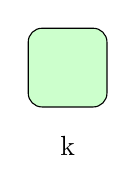
\begin{tikzpicture}[scale=1]
      % \draw[help lines, gray!50, very thin] (0,0) grid (6,4);
      % \filldraw[black] (0,0) circle (2pt);

      \draw[fill=green!20, rounded corners=5pt] (0,1) rectangle node {\textbf{ }} (1,2);
      \node at (0.5,0.5) {k};
    \end{tikzpicture}
  \end{center}

  \begin{verbatim}
  int k;
  \end{verbatim}

  \framebreak

  \begin{center}
    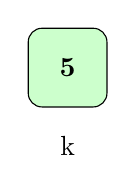
\begin{tikzpicture}[scale=1]
      % \draw[help lines, gray!50, very thin] (0,0) grid (6,4);
      % \filldraw[black] (0,0) circle (2pt);

      \draw[fill=green!20, rounded corners=5pt] (0,1) rectangle node {\textbf{5}} (1,2);
      \node at (0.5,0.5) {k};
    \end{tikzpicture}
  \end{center}

  \begin{verbatim}
  int k;
  k = 5;
  \end{verbatim}

  \framebreak

  \begin{center}
    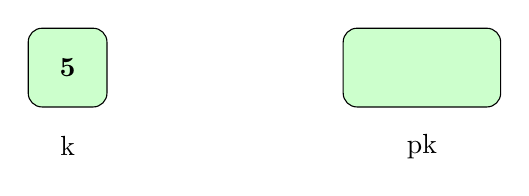
\begin{tikzpicture}[scale=1]
      % \draw[help lines, gray!50, very thin] (0,0) grid (6,4);
      % \filldraw[black] (0,0) circle (2pt);

      \draw[fill=green!20, rounded corners=5pt] (0,1) rectangle node {\textbf{5}} (1,2);
      \node at (0.5,0.5) {k};
      \draw[fill=green!20, rounded corners=5pt] (4,1) rectangle node {\textbf{ }} (6,2);
      \node at (5.0,0.5) {pk};
    \end{tikzpicture}
  \end{center}

  \begin{verbatim}
  int k;
  k = 5;
  int *pk;
  \end{verbatim}
  
  \framebreak

  \begin{center}
    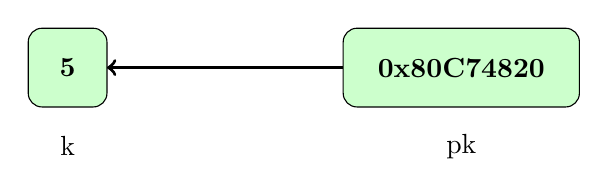
\begin{tikzpicture}[scale=1]
      % \draw[help lines, gray!50, very thin] (0,0) grid (6,4);
      % \filldraw[black] (0,0) circle (2pt);

      \draw[fill=green!20, rounded corners=5pt] (0,1) rectangle node {\textbf{5}} (1,2);
      \node at (0.5,0.5) {k};
      \draw[fill=green!20, rounded corners=5pt] (4,1) rectangle node {\textbf{0x80C74820}} (7,2);
      \node at (5.5,0.5) {pk};
      \draw[->, very thick] (4,1.5) -- (1,1.5);
    \end{tikzpicture}
  \end{center}

  \begin{verbatim}
  int k;
  k = 5;
  int *pk;
  pk = &k;
  \end{verbatim}
  
  \framebreak

  Um ponteiro é apenas uma variável cujo valor é um endereço de
  memória. O tipo descreve o dado localizado no endereço.

  O ponteiro mais simples de C é o NULL. O NULL aponta para nenhum
  lugar, o que será bastante útil. O elemento neutro.

  Ao criar um ponteiro, se um valor não for atribuído imediatamente
  (um endereço), é adequado sempre atribuir o valor NULL.

  Você pode verificar se o ponteiro é NULL com o operador de igualdade
  (\ilcode{==}).

  \framebreak

  A forma mais fácil de obter um ponteiro é extrair o endereço de uma
  variável já existente, para isso usamos o operador \ilcode{\&}.

  Se \ilcode{x} for uma variável do tipo \ilcode{int}, então
  \ilcode{\&x} é o endereço de \ilcode{x}. E podemos criar um ponteiro
  para \ilcode{x} com valor igual a \ilcode{\&x}.

  Se \ilcode{arr} é um array de doubles, então \ilcode{\&arr[i]} é um
  ponteiro para double cujo valor é o endereço do iéssimo elemento de
  \ilcode{arr}.

  O nome de um array é basicamente um ponteiro para o seu primeiro
  elemento.

  \framebreak

  Com ponteiros, temos uma forma altenativa de passar dados para
  funções. 

  Até agora, valores eram passados \textbf{por valor}, o que significa
  que uma cópia do valor armazenado na variável referenciada na
  chamada da função era passada.

  A única excessão até agora ocorria com arrays.

  \framebreak

  Usando ponteiros, podemos passar a variável sendo referenciada na
  chamada, ou melhor, uma referência à ela, seu endereço.

  Isto significa que uma mudança feita na variável no corpo da função
  chamada irá mudar o valor da variável mesmo quando a função chamada
  retornar.

  Isto pode ser bom ou ruim! Teremos que ter mais cuidado.

  \framebreak

  Para inspecionar ou modificar um determinado endereço da memória
  apontada por um ponteiro precisamos \textbf{dereferenciando} o
  ponteiro.

  Se tivermos um ponteiro chamado \ilcode{pc}, então \ilcode{*pc} é o
  valor que está armazenado no endereço da memória armazenado na
  variável \ilcode{pc}.

  \framebreak

  Então existem dois contextos de uso do operador \ilcode{*}. Como
  \textbf{dereferenciador}, ele 'vai para a referência' e acessa o
  dado que estiver naquela localização da memória.

  Se tentarmos \textbf{dereferenciar} um ponteiro cujo valor é
  \ilcode{NULL}, teremos um

  \begin{center}
    {\color{red} Segmentation fault}
  \end{center}
  
  Isto, na verdade, é um comportamento esperado. É uma defesa contra
  um acesso indesejado a um ponteiro desconhecido.

  \framebreak

  Mais uma coisa irritante sobre o operador \ilcode{*}. Ele é parte
  tanto do tipo quanto do nome de uma variável.

  \lstinputlisting[style=normalc,caption=src/decl.c]{src/decl.c}
  
  \framebreak

  \begin{center}
    \begin{tabular}{cc}
      \hline
      Data Type & Size (in bytes)\\
      \hline
      int & 4\\
      char & 1\\
      float & 4\\
      double & 8\\
      long long & 8\\
      char*, int*, double*, float* \ldots & 8\\
      \hline
    \end{tabular}
  \end{center}

\end{frame}
  

\begin{frame}[allowframebreaks,fragile]{passo a passo}
    
  \begin{center}
    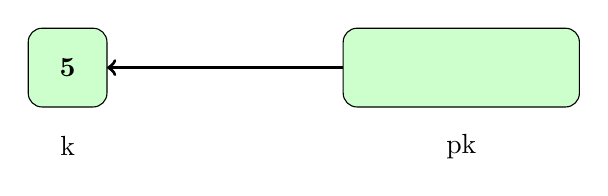
\begin{tikzpicture}[scale=1]
      % \draw[help lines, gray!50, very thin] (0,0) grid (6,4);
      % \filldraw[black] (0,0) circle (2pt);

      \draw[fill=green!20, rounded corners=5pt] (0,1) rectangle node {\textbf{5}} (1,2);
      \node at (0.5,0.5) {k};
      \draw[fill=green!20, rounded corners=5pt] (4,1) rectangle node {\textbf{ }} (7,2);
      \node at (5.5,0.5) {pk};
      \draw[->, very thick] (4,1.5) -- (1,1.5);
    \end{tikzpicture}
  \end{center}
  
  \framebreak

  \begin{center}
    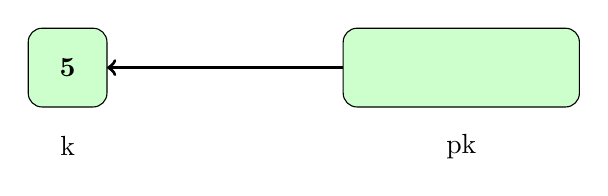
\begin{tikzpicture}[scale=1]
      % \draw[help lines, gray!50, very thin] (0,0) grid (6,4);
      % \filldraw[black] (0,0) circle (2pt);

      \draw[fill=green!20, rounded corners=5pt] (0,1) rectangle node {\textbf{5}} (1,2);
      \node at (0.5,0.5) {k};
      \draw[fill=green!20, rounded corners=5pt] (4,1) rectangle node {\textbf{ }} (7,2);
      \node at (5.5,0.5) {pk};
      \draw[->, very thick] (4,1.5) -- (1,1.5);
    \end{tikzpicture}
  \end{center}
  \begin{verbatim}
  *pk = 35;
  \end{verbatim}

  \framebreak

  \begin{center}
    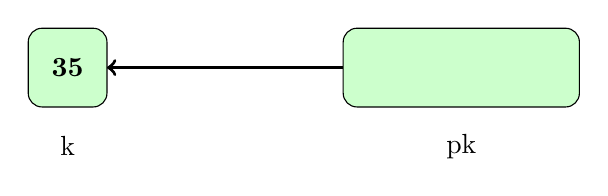
\begin{tikzpicture}[scale=1]
      % \draw[help lines, gray!50, very thin] (0,0) grid (6,4);
      % \filldraw[black] (0,0) circle (2pt);

      \draw[fill=green!20, rounded corners=5pt] (0,1) rectangle node {\textbf{35}} (1,2);
      \node at (0.5,0.5) {k};
      \draw[fill=green!20, rounded corners=5pt] (4,1) rectangle node {\textbf{ }} (7,2);
      \node at (5.5,0.5) {pk};
      \draw[->, very thick] (4,1.5) -- (1,1.5);
    \end{tikzpicture}
  \end{center}
  \begin{verbatim}
  *pk = 35;
  \end{verbatim}

  \framebreak

  \begin{center}
    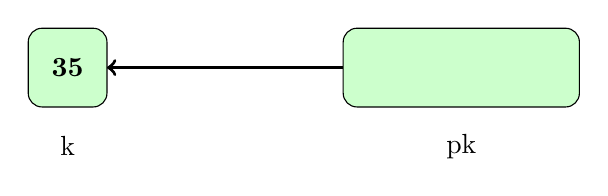
\begin{tikzpicture}[scale=1]
      % \draw[help lines, gray!50, very thin] (0,0) grid (6,4);
      % \filldraw[black] (0,0) circle (2pt);

      \draw[fill=green!20, rounded corners=5pt] (0,1) rectangle node {\textbf{35}} (1,2);
      \node at (0.5,0.5) {k};
      \draw[fill=green!20, rounded corners=5pt] (4,1) rectangle node {\textbf{ }} (7,2);
      \node at (5.5,0.5) {pk};
      \draw[->, very thick] (4,1.5) -- (1,1.5);
    \end{tikzpicture}
  \end{center}
  \begin{verbatim}
  *pk = 35;
  int m;
  \end{verbatim}

  \framebreak

  \begin{center}
    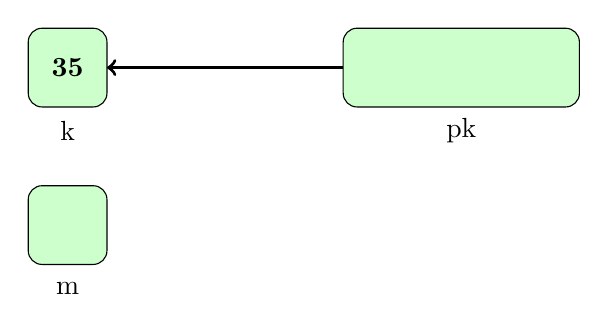
\begin{tikzpicture}[scale=1]
      % \draw[help lines, gray!50, very thin] (0,0) grid (6,4);
      % \filldraw[black] (0,0) circle (2pt);

      \draw[fill=green!20, rounded corners=5pt] (0,1) rectangle node {\textbf{35}} (1,2);
      \node at (0.5,0.7) {k};

      \draw[fill=green!20, rounded corners=5pt] (0,-1) rectangle node {\textbf{}} (1,0);
      \node at (0.5,-1.3) {m};
      
      \draw[fill=green!20, rounded corners=5pt] (4,1) rectangle node {\textbf{ }} (7,2);
      \node at (5.5,0.7) {pk};
      \draw[->, very thick] (4,1.5) -- (1,1.5);
    \end{tikzpicture}
  \end{center}
  \begin{verbatim}
  *pk = 35;
  int m;
  \end{verbatim}

  \framebreak
  
  \begin{center}
    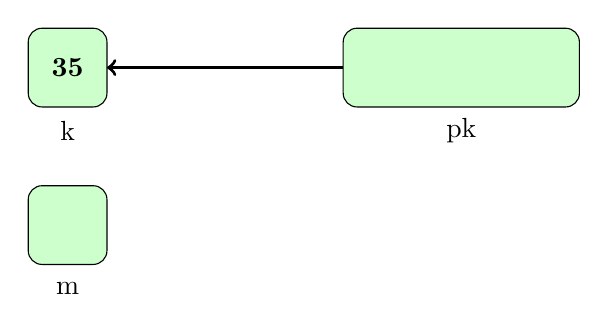
\begin{tikzpicture}[scale=1]
      % \draw[help lines, gray!50, very thin] (0,0) grid (6,4);
      % \filldraw[black] (0,0) circle (2pt);
      
      \draw[fill=green!20, rounded corners=5pt] (0,1) rectangle node {\textbf{35}} (1,2);
      \node at (0.5,0.7) {k};
      
      \draw[fill=green!20, rounded corners=5pt] (0,-1) rectangle node {\textbf{ }} (1,0);
      \node at (0.5,-1.3) {m};
      
      \draw[fill=green!20, rounded corners=5pt] (4,1) rectangle node {\textbf{ }} (7,2);
      \node at (5.5,0.7) {pk};
      \draw[->, very thick] (4,1.5) -- (1,1.5);
    \end{tikzpicture}
  \end{center}
  \begin{verbatim}
  *pk = 35;
  int m;
  m = 4;
  \end{verbatim}

  \framebreak

  \begin{center}
    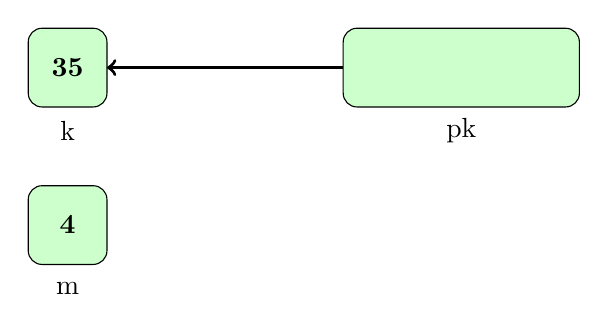
\begin{tikzpicture}[scale=1]
      % \draw[help lines, gray!50, very thin] (0,0) grid (6,4);
      % \filldraw[black] (0,0) circle (2pt);
      
      \draw[fill=green!20, rounded corners=5pt] (0,1) rectangle node {\textbf{35}} (1,2);
      \node at (0.5,0.7) {k};
      
      \draw[fill=green!20, rounded corners=5pt] (0,-1) rectangle node {\textbf{4}} (1,0);
      \node at (0.5,-1.3) {m};
      
      \draw[fill=green!20, rounded corners=5pt] (4,1) rectangle node {\textbf{ }} (7,2);
      \node at (5.5,0.7) {pk};
      \draw[->, very thick] (4,1.5) -- (1,1.5);
    \end{tikzpicture}
  \end{center}
  \begin{verbatim}
  *pk = 35;
  int m;
  m = 4;
  \end{verbatim}

  \framebreak

  \begin{center}
    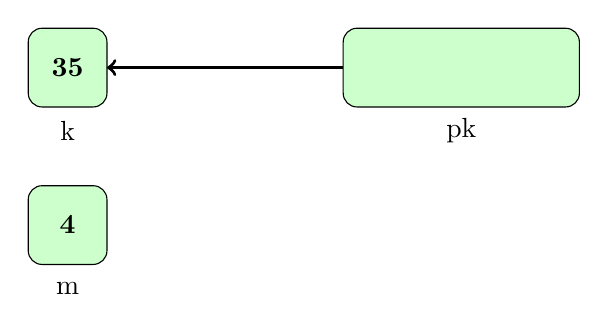
\begin{tikzpicture}[scale=1]
      % \draw[help lines, gray!50, very thin] (0,0) grid (6,4);
      % \filldraw[black] (0,0) circle (2pt);
      
      \draw[fill=green!20, rounded corners=5pt] (0,1) rectangle node {\textbf{35}} (1,2);
      \node at (0.5,0.7) {k};
      
      \draw[fill=green!20, rounded corners=5pt] (0,-1) rectangle node {\textbf{4}} (1,0);
      \node at (0.5,-1.3) {m};
      
      \draw[fill=green!20, rounded corners=5pt] (4,1) rectangle node {\textbf{ }} (7,2);
      \node at (5.5,0.7) {pk};
      \draw[->, very thick] (4,1.5) -- (1,1.5);
    \end{tikzpicture}
  \end{center}
  \begin{verbatim}
  *pk = 35;
  int m;
  m = 4;
  pk = &m;
  \end{verbatim}

  \framebreak

  \begin{center}
    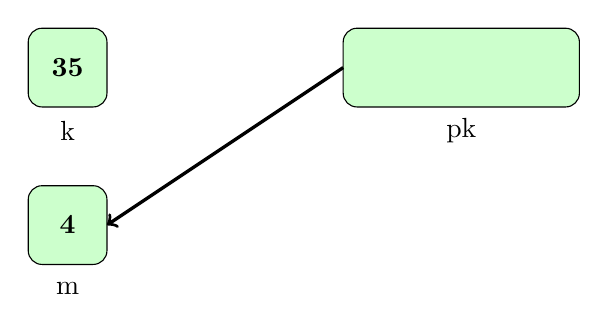
\begin{tikzpicture}[scale=1]
      % \draw[help lines, gray!50, very thin] (0,0) grid (6,4);
      % \filldraw[black] (0,0) circle (2pt);
      
      \draw[fill=green!20, rounded corners=5pt] (0,1) rectangle node {\textbf{35}} (1,2);
      \node at (0.5,0.7) {k};
      
      \draw[fill=green!20, rounded corners=5pt] (0,-1) rectangle node {\textbf{4}} (1,0);
      \node at (0.5,-1.3) {m};
      
      \draw[fill=green!20, rounded corners=5pt] (4,1) rectangle node {\textbf{ }} (7,2);
      \node at (5.5,0.7) {pk};
      \draw[->, very thick] (4,1.5) -- (1,-0.5);
    \end{tikzpicture}
  \end{center}
  \begin{verbatim}
  *pk = 35;
  int m;
  m = 4;
  pk = &m;
  \end{verbatim}
  
\end{frame}


\begin{frame}[allowframebreaks,fragile]{exemplos}
  
  O que fizemos foi preencher uma dada posição de memória, que tem um
  endereço associado, com o valor 50.

  \begin{center}
    
\includegraphics[width=.7\textwidth]{50.png}    
  \end{center}

  \framebreak

  \lstinputlisting[style=tinyc,caption=src/address01.c]{src/address01.c}

  \begin{description}
  \item[\texttt{int *p} ou \texttt{int* p}] a variável \ilcode{p} aponta para um endereço onde um valor inteiro está armazenado
  \item[\texttt{\&n}] o endereço da variável \ilcode{n}
  \item[\texttt{*p}] (\textbf{dereference operator}) retorna o valor
    armazenado no endereço armazenado em \ilcode{p}
  \end{description}

  \framebreak

  Como declaramos \ilcode{p} como sendo do tipo \ilcode{int *}, o
  compilador saberá que \ilcode{*p} é um inteiro, ou seja, o número de
  bytes que devem ser lidos.

  \begin{center}
    
\includegraphics[width=.65\textwidth]{p.png}    
  \end{center}

  Note que \ilcode{p} também tem um endereço! Observe que \ilcode{p}
  ocupa 8 bytes (64 bits).
  
\end{frame}


\end{document}

%%% Local Variables:
%%% mode: latex
%%% TeX-master: t
%%% End:
